%%----------------------------------------------------------------------------------------
\part{Momento di inerzia di una figura piana}
\setcounter{section}{0}
\section{Definizione di momento di inerzia}
%\label{paragrafo1-1}
%----------------------------------------------------------------------------------------
Con riferimento alla figura~\vref{figura1-2}, si definisce momento di inerzia rispetto alla retta $r$ la quantità:
%----------------------------------------------------------------------------------------
\begin{equation} \label{equazione2-1}
I_r = \int\int_A \lambda^2dA \tag{2.1}
\end{equation}
%----------------------------------------------------------------------------------------
Nel caso di figura~\ref{figura1-3}, la precedente relazione si particolarizza nelle:
%----------------------------------------------------------------------------------------
\begin{align}
I_x &= \int\int_A y^{2}dA \tag{2.2a} \label{equazione2-2a} \\ 
I_y &= \int\int_A x^{2}dA \tag{2.2b} \label{equazione2-2b}
\end{align}
%----------------------------------------------------------------------------------------
È ovvio che $I_r$ è sempre maggiore di zero ($I_r>0$) e le sue dimensioni fisiche sono $[L^4]$.
%----------------------------------------------------------------------------------------
\section{Formule notevoli di momenti di inerzia}
%----------------------------------------------------------------------------------------
\renewcommand{\thefigure}{2~-~1}
\begin{figure}[ht]
\centering
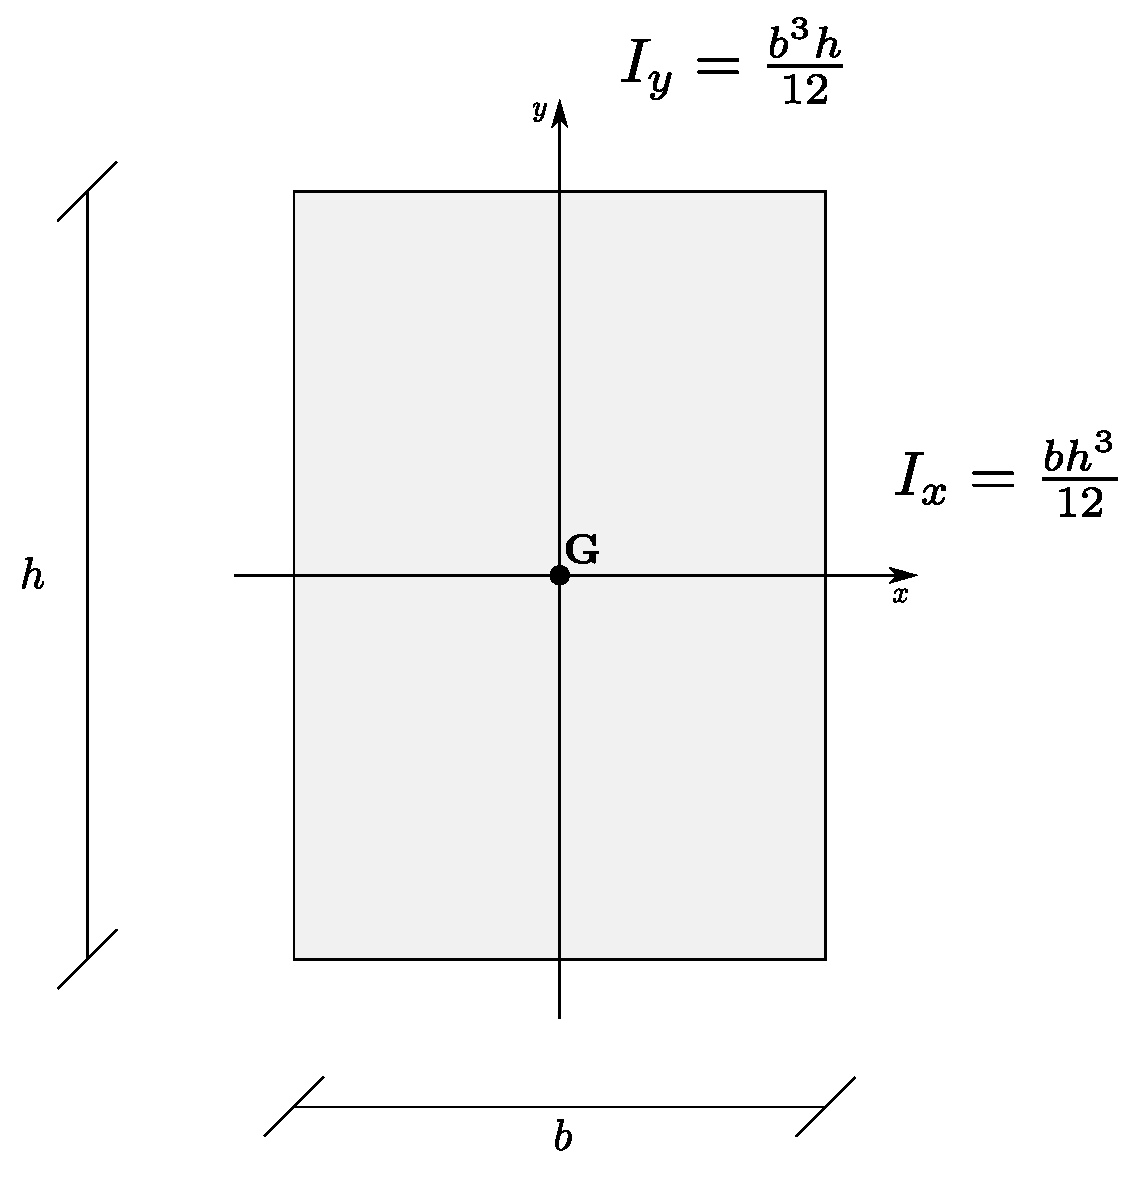
\includegraphics[width=0.55\textwidth]{Immagini/Parte_2/Figura2_1/Figura2_1.pdf}
\caption{}
\label{figura2-1}
\end{figure}
%----------------------------------------------------------------------------------------
%---------------------------------------------------------------------------------------------------------------------------------------------
\begin{align}
I_x &= \frac{bh^{3}}{12} \tag{2.3a} \label{equazione2-3a} \\
I_y &= \frac{b^{3}h}{12} \tag{2.3b} \label{equazione2-3b}
\end{align}
%---------------------------------------------------------------------------------------------------------------------------------------------
Limitiamoci a dimostrare la relazione per il calcolo di $I_x$. 
%----------------------------------------------------------------------------------------
\begin{equation*}
I_x = \int\int_A y^{2}dA = \int_{-\frac{b}{2}}^{+\frac{b}{2}}dx\int_{-\frac{h}{2}}^{+\frac{h}{2}}y^{2}dy = \bigl[x\bigr]_{-\frac{b}{2}}^{+\frac{b}{2}}\cdot \frac{1}{3}\bigl[y^3\bigr]_{-\frac{h}{2}}^{+\frac{h}{2}} = \frac{bh^3}{12}
\end{equation*}
%----------------------------------------------------------------------------------------
%----------------------------------------------------------------------------------------
\renewcommand{\thefigure}{2~-~2}
\begin{figure}[ht]
\centering
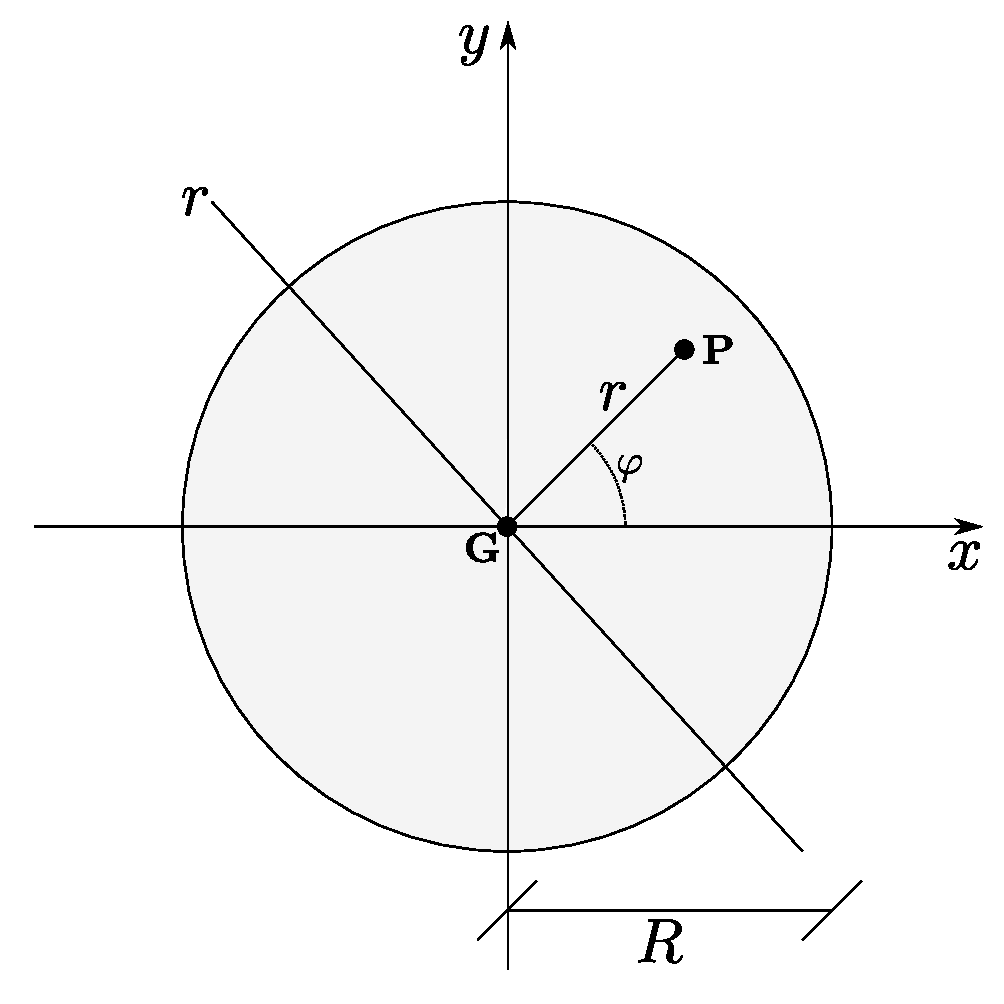
\includegraphics[width=0.58\textwidth]{Immagini/Parte_2/Figura2_2/Figura2_2.pdf}
\caption{}
\label{figura2-2}
\end{figure}
%----------------------------------------------------------------------------------------
È evidente che nel caso di un cerchio
%----------------------------------------------------------------------------------------
\begin{equation*}
I_r = I_x = I_y, \quad \forall r \owns \mathbf{G}
\end{equation*}
%----------------------------------------------------------------------------------------
Dimostreremo che 
%----------------------------------------------------------------------------------------
\begin{equation} \label{equazione2-4}
\boxed{I_x = \frac{\pi R^4}{4}}
\tag{2.4}
\end{equation}
%----------------------------------------------------------------------------------------
\begin{equation*}
I_x = \int\int_A y^{2}dxdy = \int\int_A (r\sin\varphi)^{2}rd\varphi dr = \int_{0}^{R}r^{3}dr\int_{0}^{2\pi}\sin^{2}\varphi d\varphi = \frac{R^4}{4}\biggl[\frac{1}{2}\varphi-\frac{1}{4}\sin 2\varphi \biggr]_{0}^{2\pi}
\end{equation*}
%----------------------------------------------------------------------------------------
che verifica la~\eqref{equazione2-4}.
%----------------------------------------------------------------------------------------
%----------------------------------------------------------------------------------------
\renewcommand{\thefigure}{2~-~3}
\begin{figure}[ht]
\centering
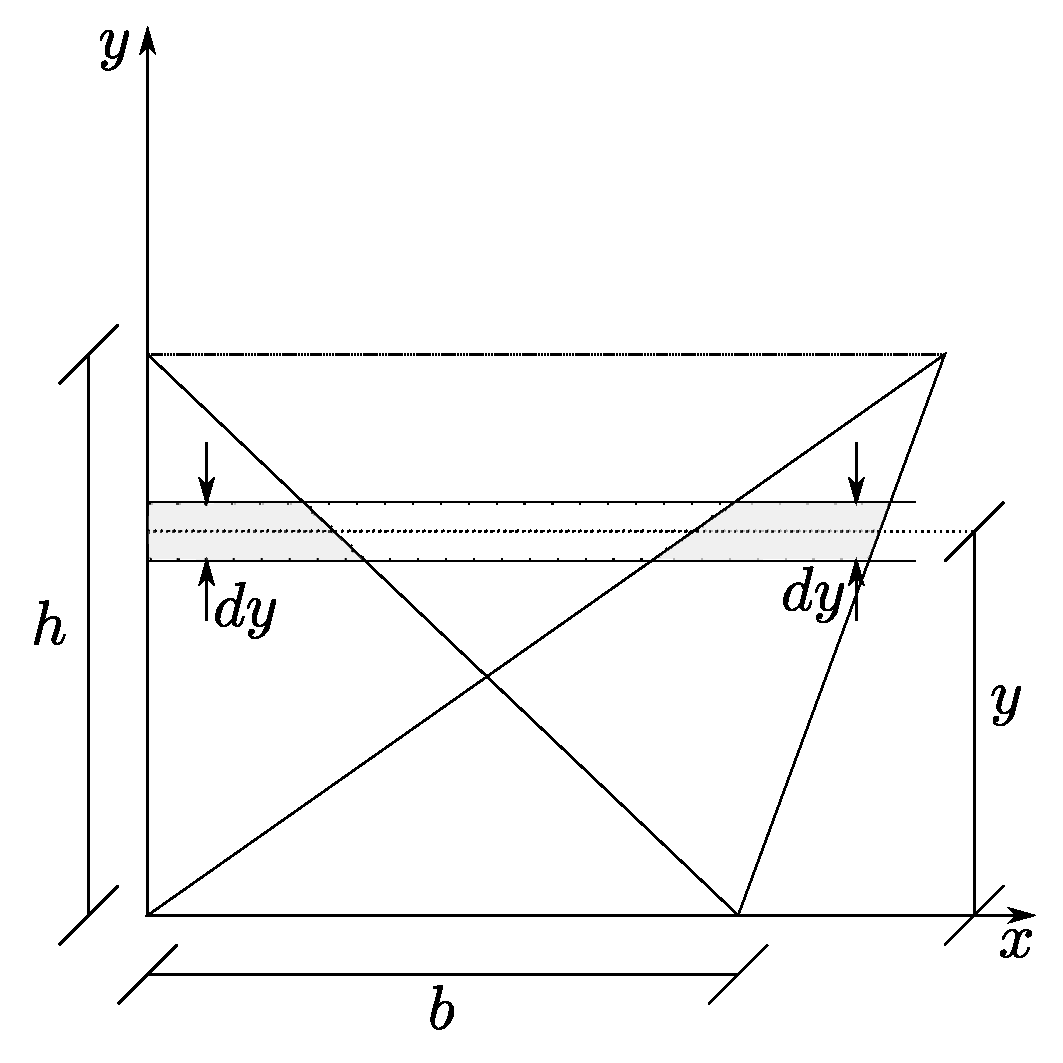
\includegraphics[width=0.75\textwidth]{Immagini/Parte_2/Figura2_3/Figura2_3.pdf}
\caption{}
\label{figura2-3}
\end{figure}
%----------------------------------------------------------------------------------------
\noindent In figura~\ref{figura2-3} sono riportati un triangolo rettangolo ed uno scaleno aventi in comune la base $b$ e l'altezza $h$. È interessante osservare che due striscette ombreggiate di spessore $dy$ hanno, a parità di quota $y$, la stessa lunghezza e quindi la stessa area $dA$. Il momento di inerzia rispetto alla retta coincidente con la base (asse $x$ in figura) è dunque uguale per entrambi. Nel caso del triangolo rettangolo è facile calcolare l'integrale:
%----------------------------------------------------------------------------------------
\begin{equation*}
I_x = \int\int_A y^{2}dxdy
\end{equation*}
%----------------------------------------------------------------------------------------
Si lascia al lettore il compito di verificare che l'equazione~\eqref{equazione2-3a} è valida per qualunque triangolo di altezza $h$ e base $b$, se $x$ coincide con la base.
%----------------------------------------------------------------------------------------

\noindent Per il triangolo rettangolo risulta chiaramente 
%----------------------------------------------------------------------------------------
\begin{equation*}
I_y = \frac{hb^{3}}{12}
\end{equation*}
%----------------------------------------------------------------------------------------
È ovvio che quest'ultima formula non è valida per il triangolo scaleno; per esso sarà certamente $I_y > \frac{hb^{3}}{12}$; e, comunque, impareremo a calcolarlo in seguito. 
%----------------------------------------------------------------------------------------
%----------------------------------------------------------------------------------------
\renewcommand{\thefigure}{2~-~4}
\begin{figure}[ht]
\centering
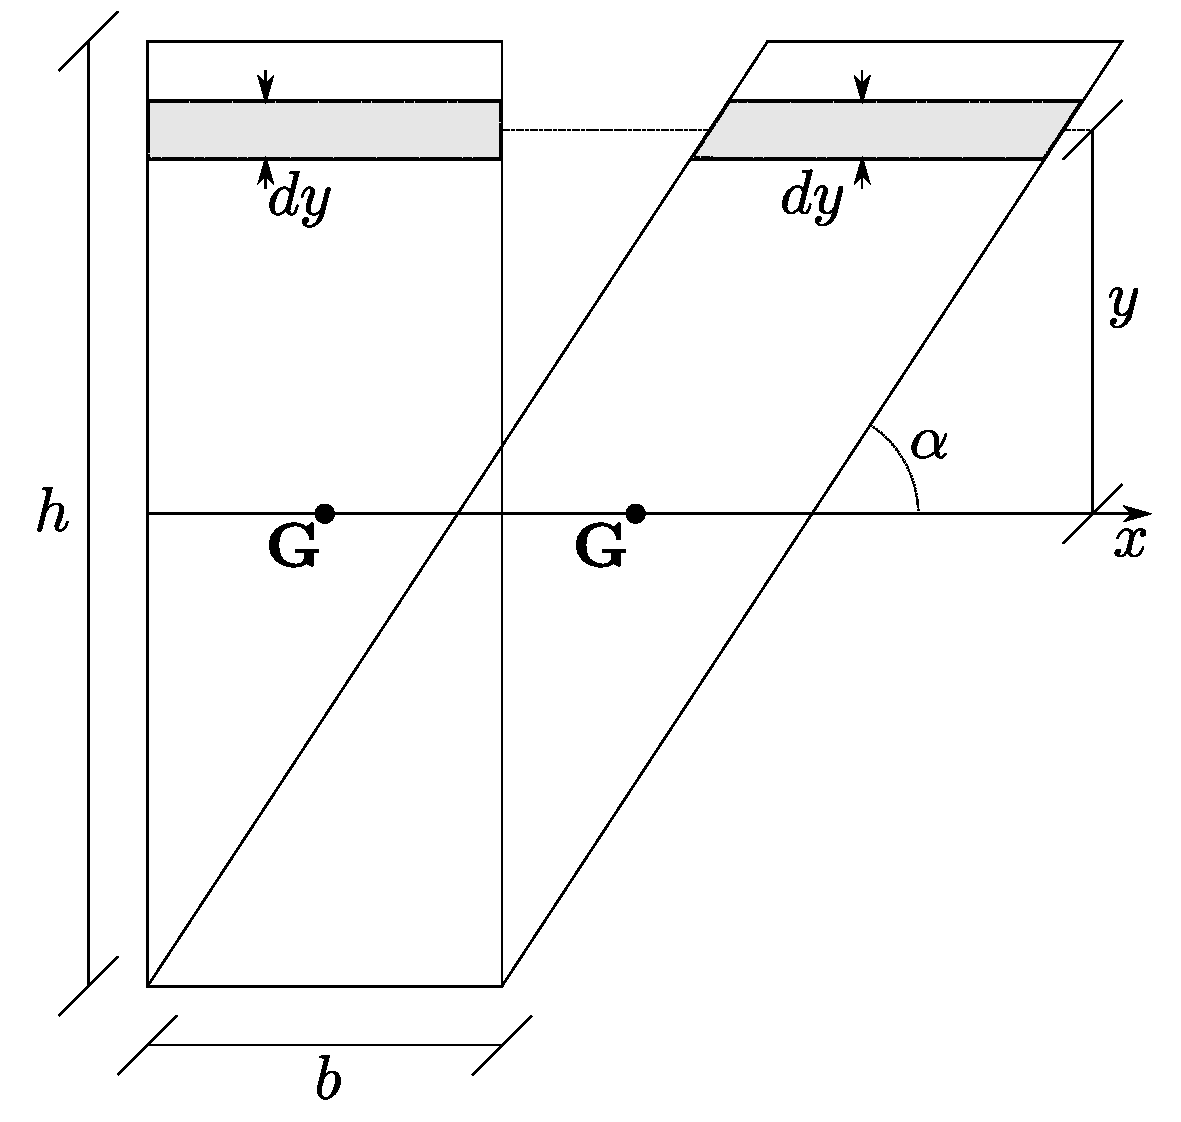
\includegraphics[width=0.75\textwidth]{Immagini/Parte_2/Figura2_4/Figura2_4.pdf}
\caption{}
\label{figura2-4}
\end{figure}
%----------------------------------------------------------------------------------------
\noindent In figura~\ref{figura2-4} sono riportati un rettangolo ed un parallelogramma aventi base ed altezza uguali. È evidente che le due striscette ombreggiate hanno la stessa area $bdy$; il momento di inerzia rispetto ad $x$ è, pertanto, uguale per entrambi. 
%----------------------------------------------------------------------------------------

\noindent Possiamo pertanto affermare che il momento di inerzia di un parallelogramma rispetto all'asse baricentrico parallelo alle basi vale, qualunque sia il valore dell'angolo $\alpha$:
%----------------------------------------------------------------------------------------
\begin{equation*}
I_x = \frac{bh^{3}}{12}
\end{equation*}
%----------------------------------------------------------------------------------------
\section{Momento di inerzia polare}
%----------------------------------------------------------------------------------------
\renewcommand{\thefigure}{2~-~5}
\begin{figure}[ht]
\centering
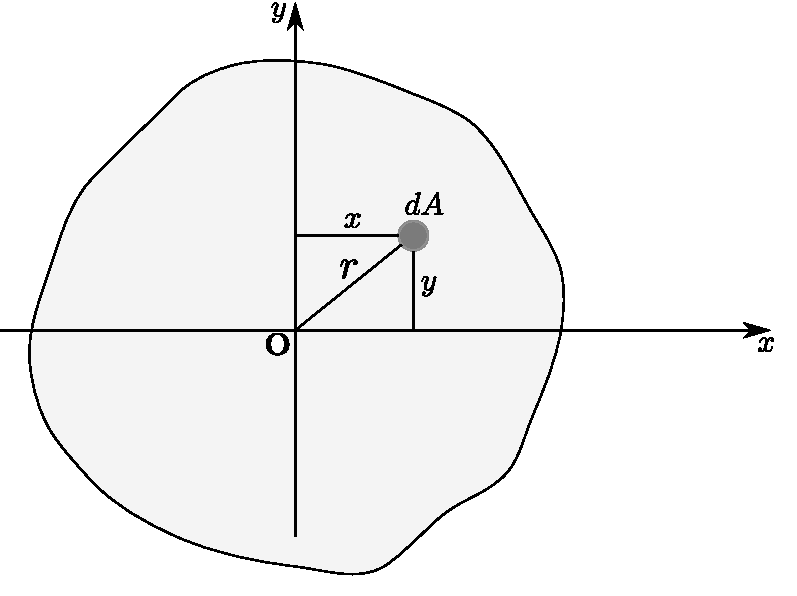
\includegraphics[width=0.75\textwidth]{Immagini/Parte_2/Figura2_5/Figura2_5.pdf}
\caption{}
\label{figura2-5}
\end{figure}
%----------------------------------------------------------------------------------------
In figura~\ref{figura2-5} è rappresentata una figura piana; $\mathbf{O}$ è un punto qualunque ad essa complanare; diciamo $r$ la distanza della generica areola $dA$ dal punto $\mathbf{O}$. 
%----------------------------------------------------------------------------------------

\noindent Si dice momento di inerzia polare della figura rispetto al polo $\mathbf{O}$ la quantità:
%----------------------------------------------------------------------------------------
\begin{equation} \label{equazione2-5}
\boxed{I_x = \int\int_A r^{2}dA}
\tag{2.5}
\end{equation}
%----------------------------------------------------------------------------------------
Presi comunque due assi di riferimento ortogonali con origine in $\mathbf{O}$, sarà ovviamente: 
%----------------------------------------------------------------------------------------
\begin{equation*}
r^2 = x^2 + y^2
\end{equation*}
%----------------------------------------------------------------------------------------
e pertanto la~\eqref{equazione2-5} diviene
%----------------------------------------------------------------------------------------
\begin{equation*}
I_p = \int\int_A (x^2+y^2)dA = \int\int_A x^{2}dA + \int\int_A y^{2}dA
\end{equation*}
%----------------------------------------------------------------------------------------
cioè
%----------------------------------------------------------------------------------------
\begin{equation} \label{equazione2-6}
\boxed{I_p = I_x + I_y}
\tag{2.6}
\end{equation}
%----------------------------------------------------------------------------------------
Ribadiamo che la~\eqref{equazione2-6} è valida comunque si prendano $x$ ed $y$, purché ortogonali e con origine nel polo.
%----------------------------------------------------------------------------------------
\section{Teorema del trasporto del momento di inerzia}
%----------------------------------------------------------------------------------------
\renewcommand{\thefigure}{2~-~6}
\begin{figure}[ht]
\centering
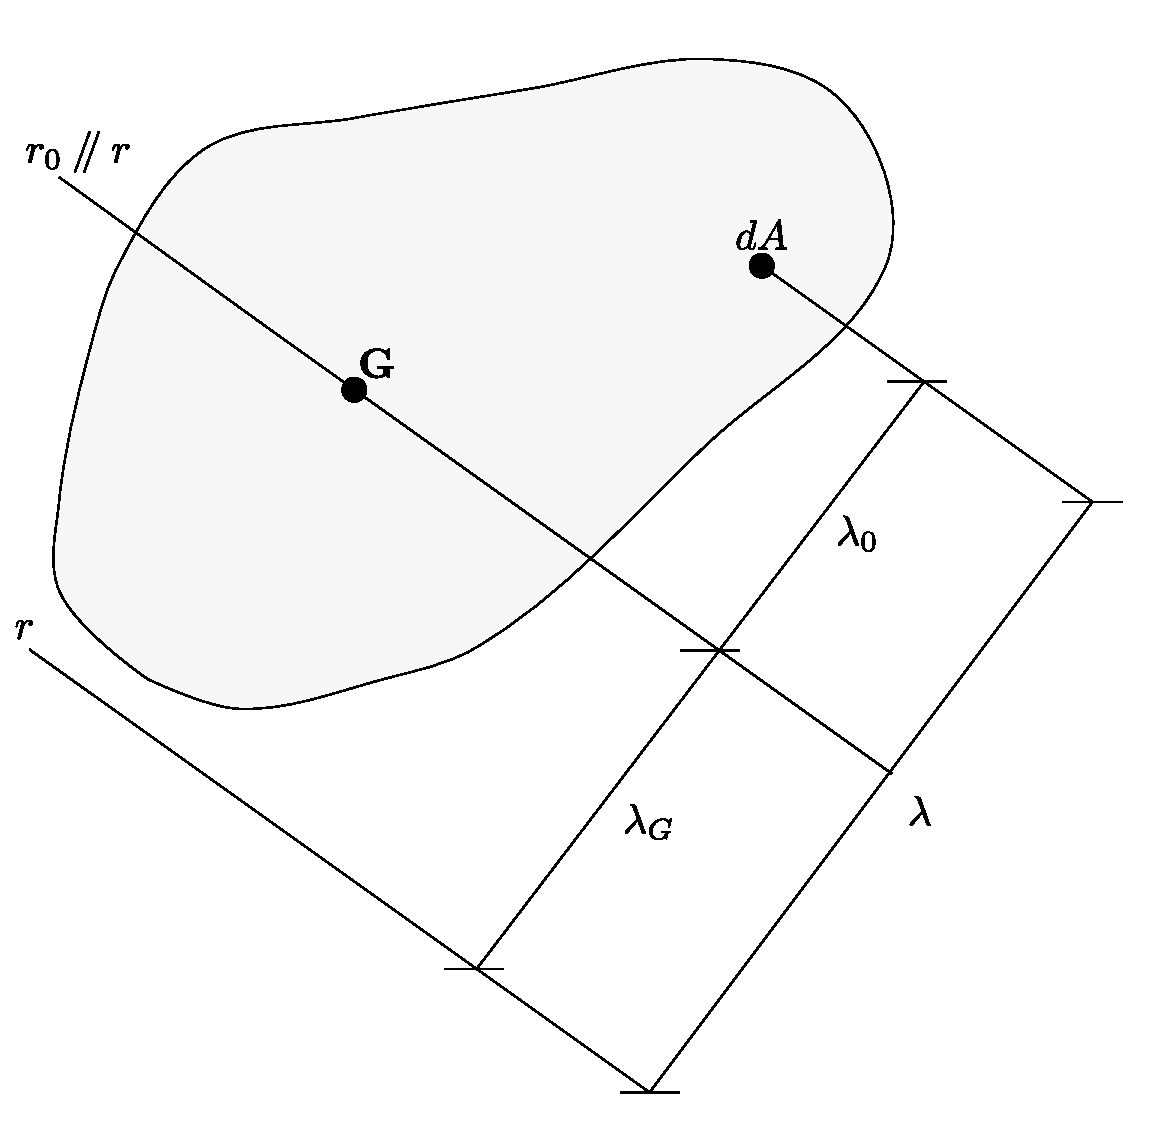
\includegraphics[width=0.75\textwidth]{Immagini/Parte_2/Figura2_6/Figura2_6.pdf}
\caption{}
\label{figura2-6}
\end{figure}
%----------------------------------------------------------------------------------------
%----------------------------------------------------------------------------------------
Dimostreremo che, qualunque, sia la figura piana e qualunque sia la retta $r$, vale la relazione:
%----------------------------------------------------------------------------------------
\begin{equation} \label{equazione2-7}
\boxed{I_r = I_{r_0}+A\lambda_{G}^{2}}
\tag{2.7}
\end{equation}
%----------------------------------------------------------------------------------------
La~\eqref{equazione2-7} esprime il \textsc{Teorema di Huygens}; il termine $A\lambda_{G}^{2}$ è detto \emph{termine di trasporto}. Per dimostrare la~\eqref{equazione2-7} cominciamo ad osservare che, come è evidente in figura~\ref{figura2-6}, risulta:
%----------------------------------------------------------------------------------------
\begin{equation*}
\lambda = \lambda_0+\lambda_G
\end{equation*}
%----------------------------------------------------------------------------------------
Ciò premesso
%----------------------------------------------------------------------------------------
\begin{equation*}
I_r = \int\int_A \lambda^{2}dA = \int\int_A (\lambda_0+\lambda_G)^{2}dA = \int\int_A \lambda_{0}^{2}dA + \int\int_A \lambda_{G}^{2}dA + \int\int_A 2\lambda_{0}\lambda_{G}dA
\end{equation*}
%----------------------------------------------------------------------------------------
Essendo $\lambda_G=\textup{\textsc{costante}}$
%----------------------------------------------------------------------------------------
\begin{equation*}
I_r = \int\int_A \lambda_{0}^{2}dA + \lambda_{G}^{2}\int\int_AdA + 2\lambda_{G}\int\int_A \lambda_{0}dA
\end{equation*}
%----------------------------------------------------------------------------------------
Ovviamente risulta 
%----------------------------------------------------------------------------------------
\begin{align*}
\int\int_A dA &= A \\
\int\int_A \lambda_{0}^{2}dA &= I_{r_0} \\
\int\int_A \lambda_{0}dA &= S_{r_0} = 0\,\,\textup{essendo}\,\,r_0\,\owns\,\mathbf{G}
\end{align*}
%----------------------------------------------------------------------------------------
e così si perviene alla~\eqref{equazione2-7}.
%----------------------------------------------------------------------------------------
\section{Altre formule notevoli di momento di inerzia}
%----------------------------------------------------------------------------------------
\renewcommand{\thefigure}{2~-~7}
\begin{figure}[ht]
\centering
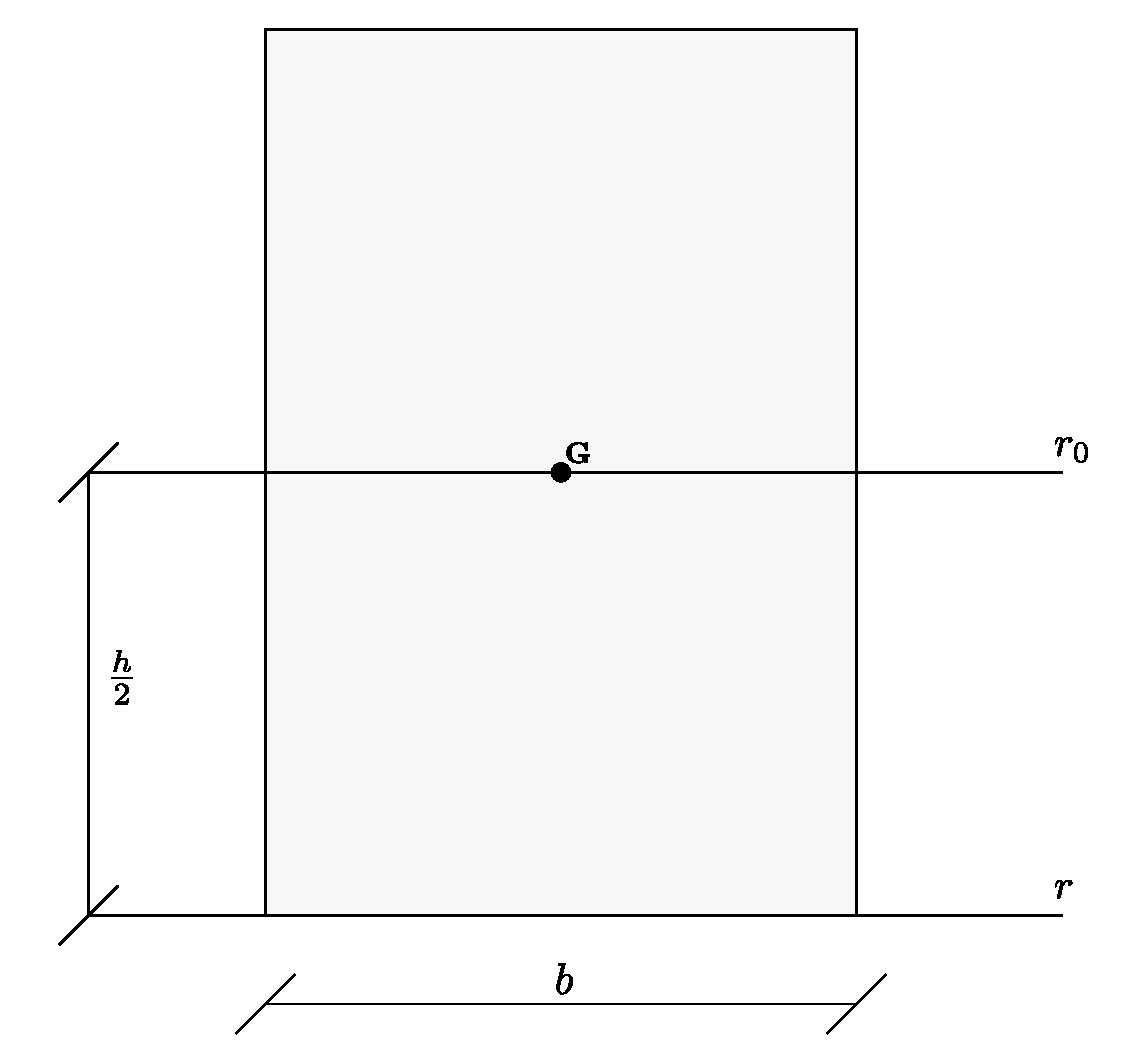
\includegraphics[width=0.75\textwidth]{Immagini/Parte_2/Figura2_7/Figura2_7.pdf}
\caption{}
\label{figura2-7}
\end{figure}
%----------------------------------------------------------------------------------------
%----------------------------------------------------------------------------------------
Con riferimento al rettangolo di figura~\ref{figura2-7} vogliamo calcolare $I_r$. Applicando il teorema del trasporto: 
%----------------------------------------------------------------------------------------
\begin{equation*}
I_r = I_{r_0}+A\lambda_{G}^{2} = \frac{bh^{3}}{12}+bh\biggl(\frac{h}{2}\biggr)^2
\end{equation*}
%----------------------------------------------------------------------------------------
e semplificando 
%----------------------------------------------------------------------------------------
\begin{equation} \label{equazione2-8}
\boxed{I_r = \frac{bh^{3}}{3}}
\tag{2.8}
\end{equation}
%----------------------------------------------------------------------------------------
%----------------------------------------------------------------------------------------
\renewcommand{\thefigure}{2~-~8}
\begin{figure}[ht]
\centering
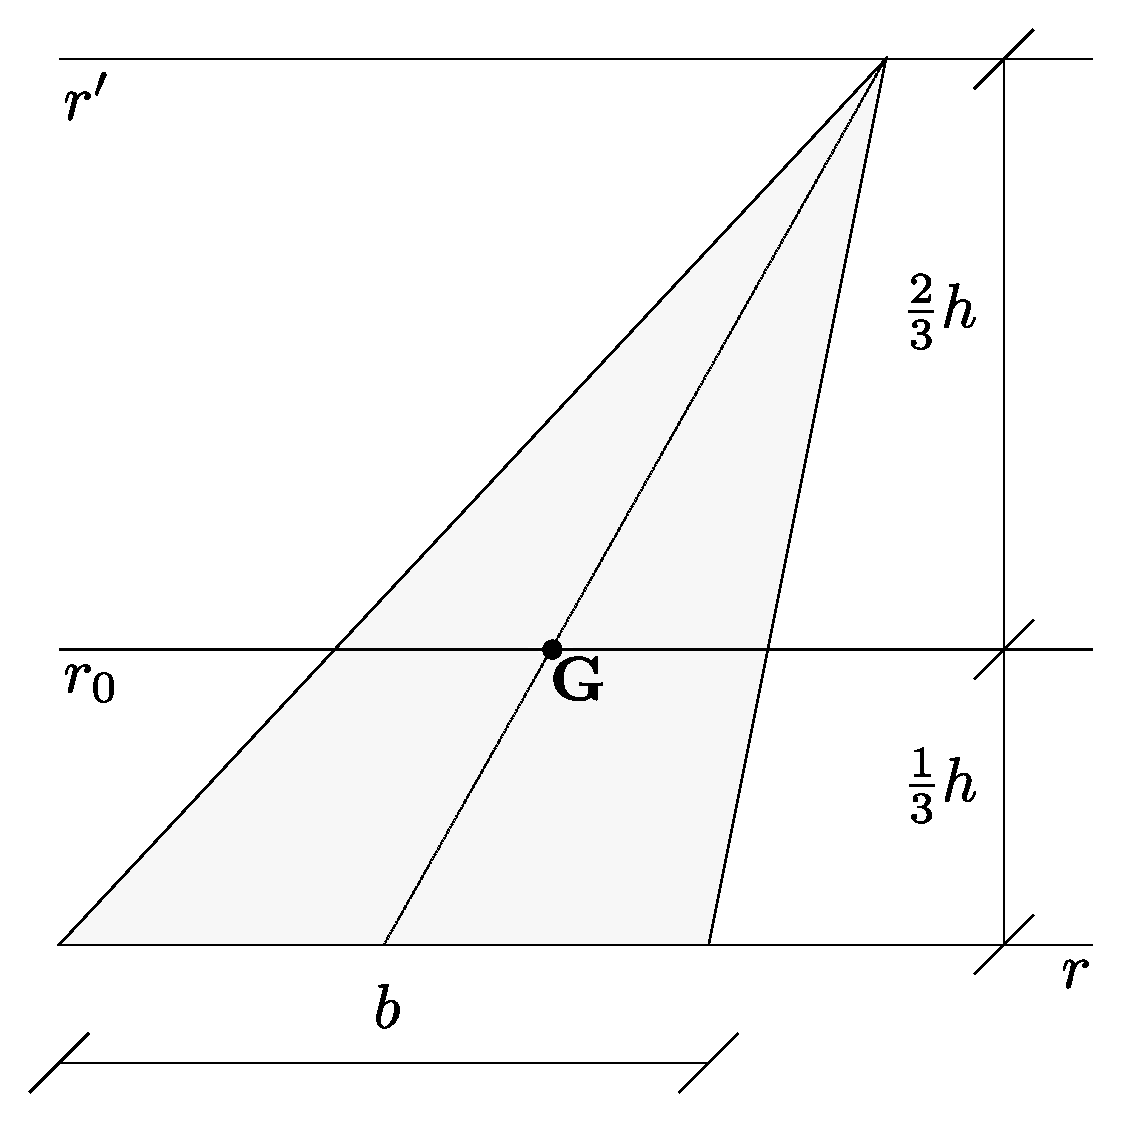
\includegraphics[width=0.75\textwidth]{Immagini/Parte_2/Figura2_8/Figura2_8.pdf}
\caption{}
\label{figura2-8}
\end{figure}
%----------------------------------------------------------------------------------------
Con riferimento al triangolo di figura~\ref{figura2-8} è noto che 
%----------------------------------------------------------------------------------------
\begin{equation*}
I_r = \frac{bh^{3}}{12}
\end{equation*}
%----------------------------------------------------------------------------------------
Ci proponiamo di calcolare $I_{r_0}$ ed $I_{r'}$. 
%----------------------------------------------------------------------------------------

\noindent Utilizzeremo, ovviamente, il teorema del trasporto:
%----------------------------------------------------------------------------------------
\begin{equation*}
I_{r_0} = I_r - A\lambda_{G}^{2} = \frac{bh^{3}}{12}-\frac{bh}{2}\biggl(\frac{h}{3}\biggr)^2
\end{equation*}
%----------------------------------------------------------------------------------------
semplificando
%----------------------------------------------------------------------------------------
\begin{equation}
\boxed{I_{r_0} = \frac{bh^{3}}{36}}
\end{equation}
%----------------------------------------------------------------------------------------
E ancora 
%----------------------------------------------------------------------------------------
\begin{equation*}
I_{r_0} = I_{r'} + A\lambda_{G}^{2} = \frac{bh^{3}}{36}+\frac{bh}{2}\biggl(\frac{2}{3}h\biggr)^2
\end{equation*}
%----------------------------------------------------------------------------------------
semplificando
%----------------------------------------------------------------------------------------
\begin{equation*}
\boxed{I_{r'} = \frac{bh^{3}}{4}}
\end{equation*}
%----------------------------------------------------------------------------------------
\clearpage
\section{Esercizi}
\paragraph{Esercizio 2.1}
Calcolare $I_y$ per il triangolo \textsc{abc} riportato in figura
%----------------------------------------------------------------------------------------
\renewcommand{\thefigure}{2.1~-~1}
\begin{figure}[ht]
\centering
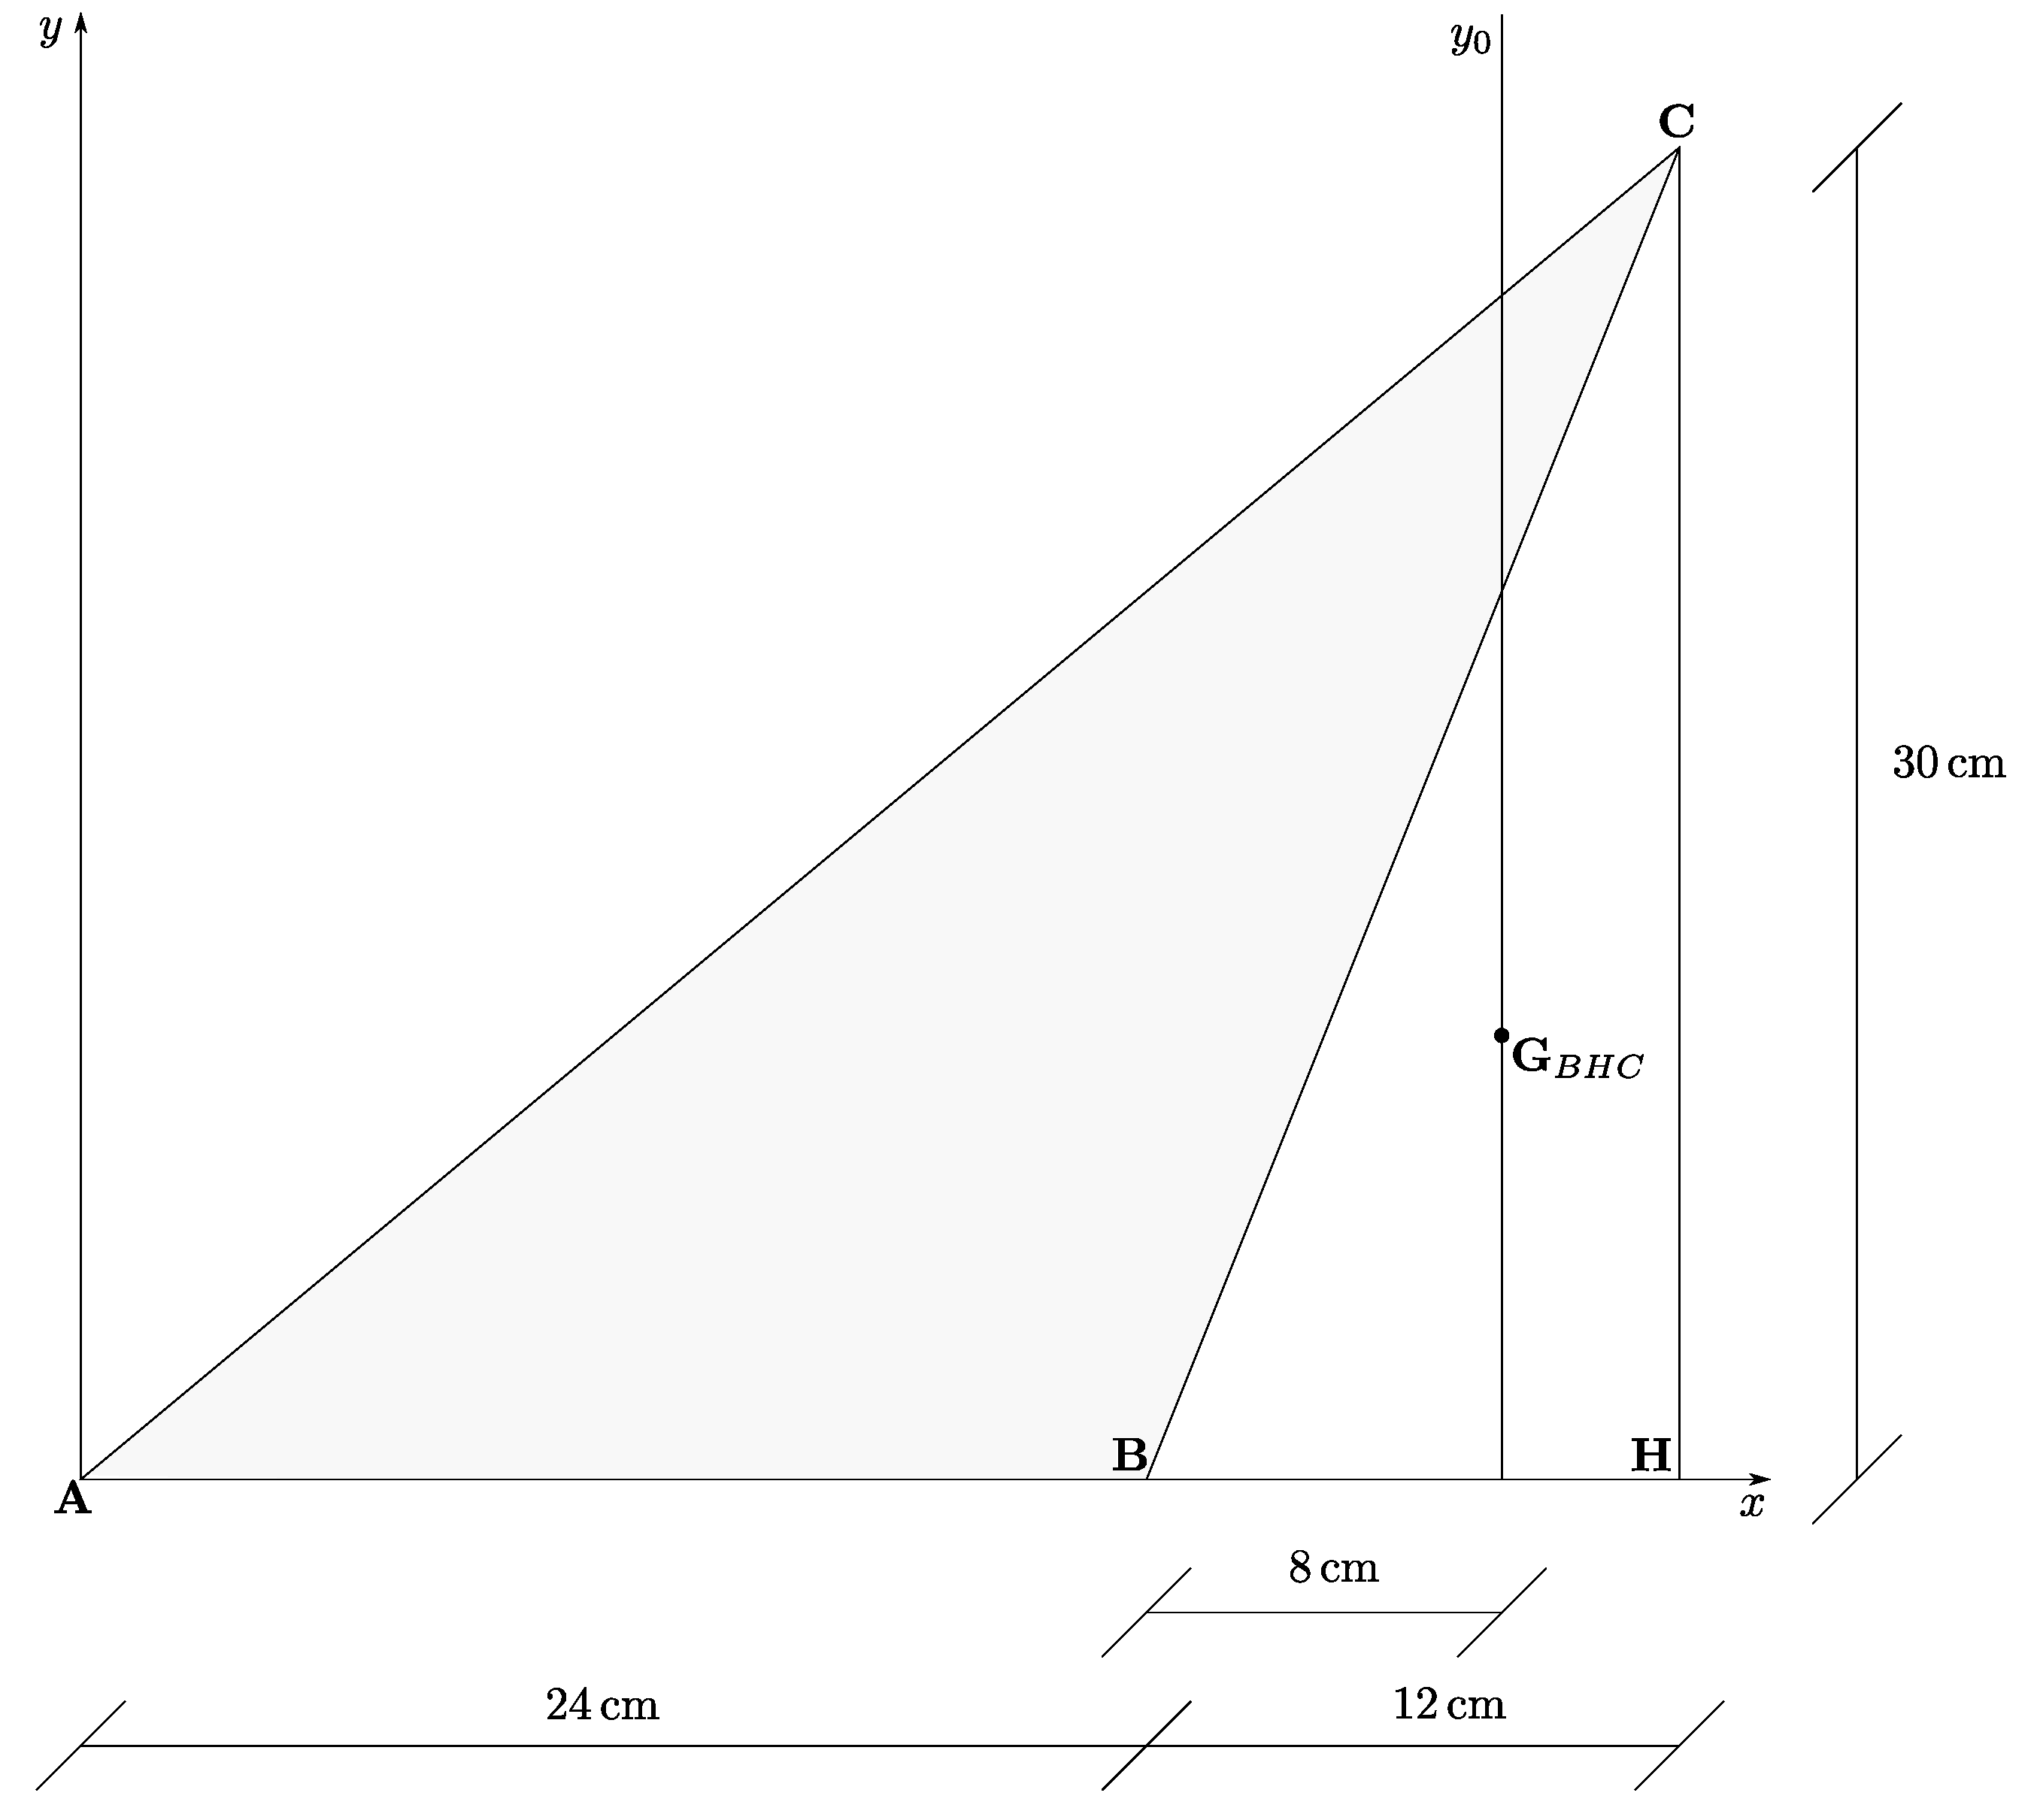
\includegraphics[width=0.95\textwidth]{Immagini/Parte_2/Esercizio2_1/Esercizio2_1_1.pdf}
\caption{}
\label{Esercizio2_1}
\end{figure}
%----------------------------------------------------------------------------------------

\noindent Chiaramente, si può porre 
%----------------------------------------------------------------------------------------
\begin{equation*}
(I_{y})_{ABC} = (I_{y})_{AHC}-(I_{y})_{BHC}
\end{equation*}
%----------------------------------------------------------------------------------------
Calcoliamo, dunque, $(I_{y})_{AHC}$ e $(I_{y})_{BHC}$:
%----------------------------------------------------------------------------------------
\begin{align*}
(I_{y})_{AHC} &= \frac{30\times 36^3}{4} = 349920\,\textup{cm}^4 \\
(I_{y})_{BHC} &= (I_{y_0})_{BHC}+A_{BHC}\times \lambda_{G}^{2} = \frac{30\times 12^3}{36}+\frac{30\times 12}{2}\times 32^2 = 185760\,\textup{cm}^4
\end{align*}
%----------------------------------------------------------------------------------------
In definitiva
%----------------------------------------------------------------------------------------
\begin{equation*}
(I_{y})_{ABC} = 349920-185760 = 164160\,\textup{cm}^4
\end{equation*}
%----------------------------------------------------------------------------------------
\clearpage
\paragraph{Esercizio 2.2}
Con riferimento alla figura piana qui rappresentata, si chiede:
%----------------------------------------------------------------------------------------
\begin{enumerate}
\item di determinare $\mathbf{G}$
\item di calcolare $I_r$
\item di calcolare $I_{r_0}$, essendo $r_0$ la retta per $\mathbf{G}$ parallela ad $r$
\end{enumerate}
%----------------------------------------------------------------------------------------
\renewcommand{\thefigure}{2.2~-~1}
\begin{figure}[ht]
\centering
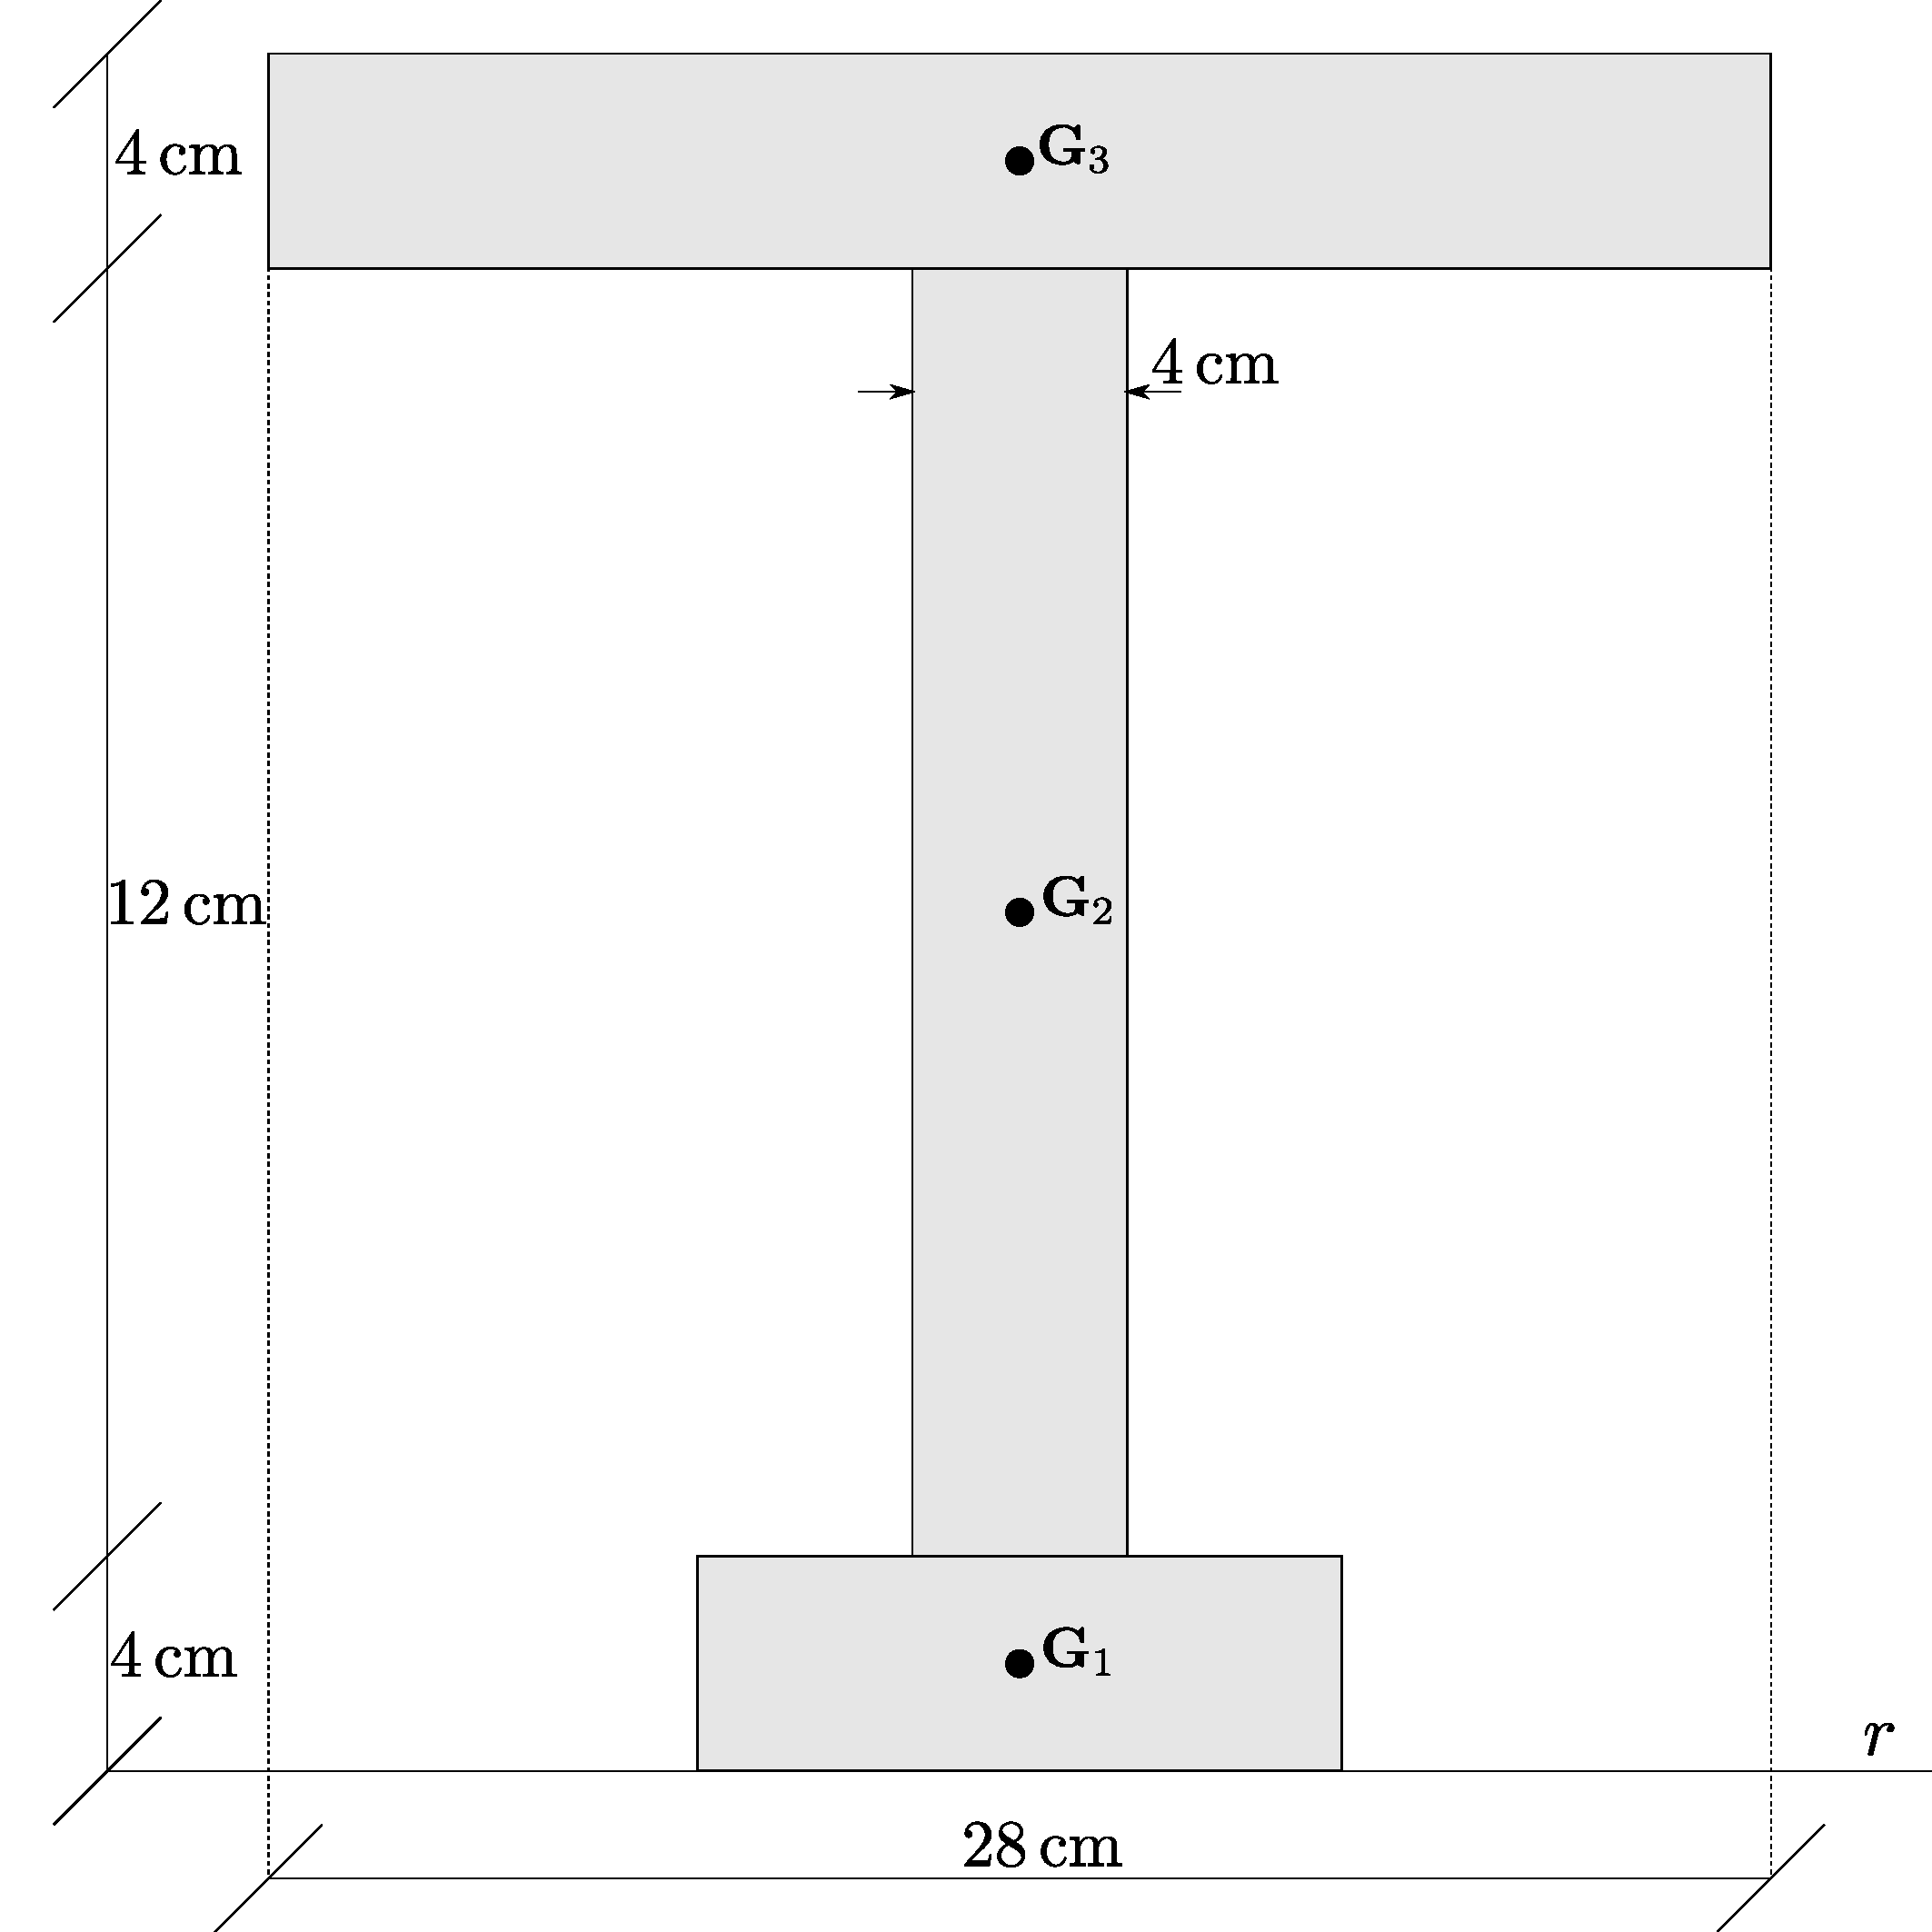
\includegraphics[width=0.95\textwidth]{Immagini/Parte_2/Esercizio2_2/Esercizio2_2_1.pdf}
\caption{}
\label{Esercizio2_1}
\end{figure}
%----------------------------------------------------------------------------------------
\noindent
\subparagraph{Quesito 1:} Il baricentro appartiene, ovviamente, all'asse di simmetria; e, perciò basterà, per determinarlo, calcolare la sua distanza da $r$.
%----------------------------------------------------------------------------------------
\begin{equation*}
\begin{aligned}
A_1 &= 12\times 4 = 48\,\textup{cm}^2 \\
A_2 &= 24\times 4 = 96\,\textup{cm}^2 \\
A_3 &= 28\times 4 = 112\,\textup{cm}^2
\end{aligned}
\,\,\Biggr\}\,\, A = 48+96+112 = 256\,\textup{cm}^2
\end{equation*}
%----------------------------------------------------------------------------------------
\begin{equation*}
\begin{aligned}
S_{1r} &= 48\times 2 = 96\,\textup{cm}^3 \\
S_{2r} &= 96\times 16 = 1536\,\textup{cm}^3 \\
S_{3r} &= 112\times 30  = 3360\,\textup{cm}^3
\end{aligned}
\,\,\Biggr\}\,\, S_r = 96+1536+3360 = 4992\,\textup{cm}^3
\end{equation*}
%----------------------------------------------------------------------------------------
\begin{equation*}
\lambda_G = \frac{S_r}{A} = \frac{4992}{256} = 19.5\,\textup{cm}
\end{equation*}
%----------------------------------------------------------------------------------------
\subparagraph{Quesito 2:} 
%----------------------------------------------------------------------------------------
\begin{equation*}
\begin{aligned}
I_{1r} &= \frac{12\times 4^{3}}{3} = 256\,\textup{cm}^4 \\
I_{2r} &= \frac{4\times 24^{3}}{12}+96\times 16^2 = 29184\,\textup{cm}^4 \\
I_{3r} &= \frac{28\times 4^{3}}{12}+112\times 30^2  = 100949\,\textup{cm}^4
\end{aligned}
\,\,\Biggr\}\,\, I_r = 256+29184+100949 = 130389\,\textup{cm}^4
\end{equation*}
%----------------------------------------------------------------------------------------
\subparagraph{Quesito 3:}
%----------------------------------------------------------------------------------------
\begin{equation*}
I_{r_0} = I_r -A\times \lambda_{G}^{2} = 130389-256\times 19.5^2 = 33045\,\textup{cm}^4
\end{equation*}
%----------------------------------------------------------------------------------------
\clearpage
\paragraph{Esercizio 2.3}
%----------------------------------------------------------------------------------------

\noindent Formulare i momenti di inerzia per il settore di corona circolare dell'Esercizio 1.3. 
%----------------------------------------------------------------------------------------
\newline

\noindent Calcoleremo gli integrali 
%----------------------------------------------------------------------------------------
\begin{align*}
I_x &= \int\int_A y^{2}dxdy \\
I_y &= \int\int_A x^{2}dxdy
\end{align*}
%----------------------------------------------------------------------------------------
Passando alle coordinate polari
%----------------------------------------------------------------------------------------
\begin{equation*}
\,\,\Biggr\{\,\, 
\begin{aligned}
x &= r\cos\varphi \\
y &= r\sin\varphi 
\end{aligned}
\quad ; \quad \lvert\, J \,\lvert = r
\end{equation*}
%----------------------------------------------------------------------------------------
si trova
%----------------------------------------------------------------------------------------
\begin{align*}
I_x &= \int\int_A r^{2}\sin^{2}\varphi rdrd\varphi = \int_{R_i}^{R_e}r^{3}dr\int_{\alpha}^{\beta}\sin^{2}\varphi d\varphi \\
I_y &= \int\int_A r^{2}\cos^{2}\varphi rdrd\varphi = \int_{R_i}^{R_e}r^{3}dr\int_{\alpha}^{\beta}\cos^{2}\varphi d\varphi
\end{align*}
%----------------------------------------------------------------------------------------
Sviluppando gli integrali si trova, infine
%----------------------------------------------------------------------------------------
\begin{align*}
I_x &= \frac{R_{e}^{4}-R_{i}^{4}}{16}(2\beta-2\alpha-\sin 2\beta+\sin 2\alpha)  \\
I_y &= \frac{R_{e}^{4}-R_{i}^{4}}{16}(2\beta-2\alpha-\sin 2\beta+\sin 2\alpha)
\end{align*}
%----------------------------------------------------------------------------------------
Le suddette formule si adattano immediatamente al caso del settore circolare ponendo in esse $R_e = R$ ed $R_i=0$.
%----------------------------------------------------------------------------------------
\clearpage
\paragraph{Esercizio 2.4}
%----------------------------------------------------------------------------------------
Formulare i momenti di inerzia per il settore di corona circolare (di spessore molto sottile) già considerato nell'Esercizio 1.7.
%----------------------------------------------------------------------------------------
\newline

\noindent Cominciamo a porre, nelle due formule di $I_x$ ed $I_y$ trovate nell'esercizio precedente 
%----------------------------------------------------------------------------------------
\begin{align*}
R_e &= r_m +\frac{\delta}{2} \\
R_i &= r_m - \frac{\delta}{2}
\end{align*}
%----------------------------------------------------------------------------------------
Osserviamo intanto che 
%----------------------------------------------------------------------------------------
\begin{equation*}
R_{e}^{4}-R_{i}^{4} = (R_{e}^{2}+R_{i}^{2})(R_{e}^{2}-R_{i}^{2}) = \Bigl(2r_{m}^{2}+\frac{\delta^2}{2}\Bigr)(2r_{m}\delta) = r_{m}\delta(4r_{m}^{2}+\delta^2)
\end{equation*}
%----------------------------------------------------------------------------------------
E quindi
%----------------------------------------------------------------------------------------
\begin{align*}
I_x &= \frac{r_{m}\delta(4r_{m}^{2}+\delta^2)}{16}(2\beta-2\alpha-\sin 2\beta+\sin 2\alpha)  \\
I_y &= \frac{r_{m}\delta(4r_{m}^{2}+\delta^2)}{16}(2\beta-2\alpha-\sin 2\beta+\sin 2\alpha)
\end{align*}
%----------------------------------------------------------------------------------------
E, trascurando $\delta^2$ rispetto a $4r_{m}^{2}$ 
%----------------------------------------------------------------------------------------
%----------------------------------------------------------------------------------------
\begin{align*}
I_x &= \frac{r_{m}^{3}\delta}{4}(2\beta-2\alpha-\sin 2\beta+\sin 2\alpha)  \\
I_y &= \frac{r_{m}^{3}\delta}{4}(2\beta-2\alpha-\sin 2\beta+\sin 2\alpha)
\end{align*}
%----------------------------------------------------------------------------------------
Nel caso $\frac{\delta}{r_m} = \frac{1}{10}$, utilizzando queste due formule, si commette un errore un po' minore dello $0.25\%$.
%----------------------------------------------------------------------------------------
\clearpage
\paragraph{Esercizio 2.5} Calcolare $I_x$ ed $I_y$ per la figura piana riportata qui rappresentata.
%----------------------------------------------------------------------------------------
\renewcommand{\thefigure}{2.5~-~1}
\begin{figure}[h]
\centering
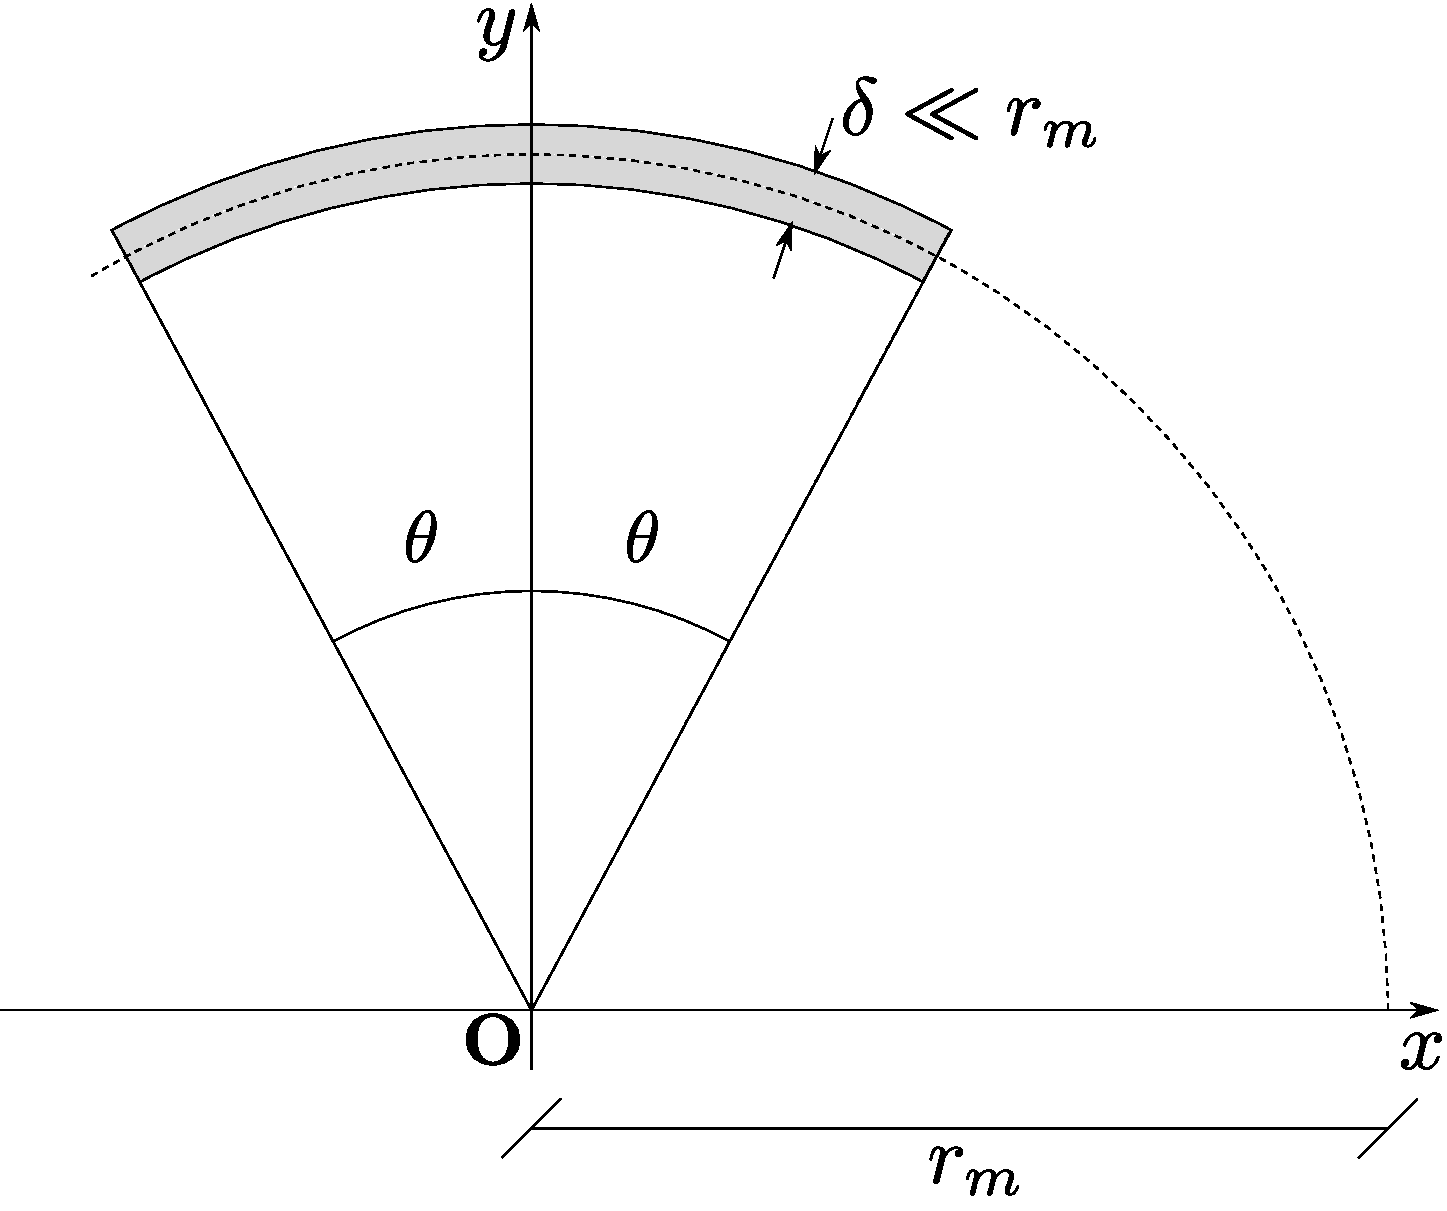
\includegraphics[width=0.85\textwidth]{Immagini/Parte_2/Esercizio2_5/Esercizio2_5_1.pdf}
\caption{}
\label{Esercizio2_5}
\end{figure}
%----------------------------------------------------------------------------------------
%----------------------------------------------------------------------------------------
\newline

\noindent Basta porre, nelle formule approssimate dell'esercizio precedente 
%----------------------------------------------------------------------------------------
\begin{align*}
\alpha &= \frac{\pi}{2} - \theta \\ 
\beta &= \frac{\pi}{2} + \theta
\end{align*}
%----------------------------------------------------------------------------------------
E così
%----------------------------------------------------------------------------------------
\begin{align*}
2\beta-2\alpha &= \pi+2\theta-(\pi-2\theta) = 4\theta \\
\sin 2\beta &= \sin(\pi+2\theta) = -\sin 2\theta \\ 
\sin 2\alpha &= \sin(\pi-2\theta) = \sin 2\theta
\end{align*}
%----------------------------------------------------------------------------------------
Pertanto
%----------------------------------------------------------------------------------------
\begin{align*}
I_x &= \frac{r_{m}^{3}\delta}{2}(2\theta+\sin 2\theta) \\ 
I_y &= \frac{r_{m}^{3}\delta}{2}(2\theta-\sin 2\theta)
\end{align*}
%----------------------------------------------------------------------------------------
%----------------------------------------------------------------------------------------
%----------------------------------------------------------------------------------------
%----------------------------------------------------------------------------------------
%----------------------------------------------------------------------------------------
%----------------------------------------------------------------------------------------
%----------------------------------------------------------------------------------------